% GNUPLOT: LaTeX picture with Postscript
\begingroup
  \makeatletter
  \providecommand\color[2][]{%
    \GenericError{(gnuplot) \space\space\space\@spaces}{%
      Package color not loaded in conjunction with
      terminal option `colourtext'%
    }{See the gnuplot documentation for explanation.%
    }{Either use 'blacktext' in gnuplot or load the package
      color.sty in LaTeX.}%
    \renewcommand\color[2][]{}%
  }%
  \providecommand\includegraphics[2][]{%
    \GenericError{(gnuplot) \space\space\space\@spaces}{%
      Package graphicx or graphics not loaded%
    }{See the gnuplot documentation for explanation.%
    }{The gnuplot epslatex terminal needs graphicx.sty or graphics.sty.}%
    \renewcommand\includegraphics[2][]{}%
  }%
  \providecommand\rotatebox[2]{#2}%
  \@ifundefined{ifGPcolor}{%
    \newif\ifGPcolor
    \GPcolortrue
  }{}%
  \@ifundefined{ifGPblacktext}{%
    \newif\ifGPblacktext
    \GPblacktextfalse
  }{}%
  % define a \g@addto@macro without @ in the name:
  \let\gplgaddtomacro\g@addto@macro
  % define empty templates for all commands taking text:
  \gdef\gplbacktext{}%
  \gdef\gplfronttext{}%
  \makeatother
  \ifGPblacktext
    % no textcolor at all
    \def\colorrgb#1{}%
    \def\colorgray#1{}%
  \else
    % gray or color?
    \ifGPcolor
      \def\colorrgb#1{\color[rgb]{#1}}%
      \def\colorgray#1{\color[gray]{#1}}%
      \expandafter\def\csname LTw\endcsname{\color{white}}%
      \expandafter\def\csname LTb\endcsname{\color{black}}%
      \expandafter\def\csname LTa\endcsname{\color{black}}%
      \expandafter\def\csname LT0\endcsname{\color[rgb]{1,0,0}}%
      \expandafter\def\csname LT1\endcsname{\color[rgb]{0,1,0}}%
      \expandafter\def\csname LT2\endcsname{\color[rgb]{0,0,1}}%
      \expandafter\def\csname LT3\endcsname{\color[rgb]{1,0,1}}%
      \expandafter\def\csname LT4\endcsname{\color[rgb]{0,1,1}}%
      \expandafter\def\csname LT5\endcsname{\color[rgb]{1,1,0}}%
      \expandafter\def\csname LT6\endcsname{\color[rgb]{0,0,0}}%
      \expandafter\def\csname LT7\endcsname{\color[rgb]{1,0.3,0}}%
      \expandafter\def\csname LT8\endcsname{\color[rgb]{0.5,0.5,0.5}}%
    \else
      % gray
      \def\colorrgb#1{\color{black}}%
      \def\colorgray#1{\color[gray]{#1}}%
      \expandafter\def\csname LTw\endcsname{\color{white}}%
      \expandafter\def\csname LTb\endcsname{\color{black}}%
      \expandafter\def\csname LTa\endcsname{\color{black}}%
      \expandafter\def\csname LT0\endcsname{\color{black}}%
      \expandafter\def\csname LT1\endcsname{\color{black}}%
      \expandafter\def\csname LT2\endcsname{\color{black}}%
      \expandafter\def\csname LT3\endcsname{\color{black}}%
      \expandafter\def\csname LT4\endcsname{\color{black}}%
      \expandafter\def\csname LT5\endcsname{\color{black}}%
      \expandafter\def\csname LT6\endcsname{\color{black}}%
      \expandafter\def\csname LT7\endcsname{\color{black}}%
      \expandafter\def\csname LT8\endcsname{\color{black}}%
    \fi
  \fi
    \setlength{\unitlength}{0.0500bp}%
    \ifx\gptboxheight\undefined%
      \newlength{\gptboxheight}%
      \newlength{\gptboxwidth}%
      \newsavebox{\gptboxtext}%
    \fi%
    \setlength{\fboxrule}{0.5pt}%
    \setlength{\fboxsep}{1pt}%
\begin{picture}(7370.00,3854.00)%
    \gplgaddtomacro\gplbacktext{%
      \csname LTb\endcsname%%
      \put(644,2350){\makebox(0,0)[r]{\strut{}0}}%
      \put(644,2643){\makebox(0,0)[r]{\strut{}0.2}}%
      \put(644,2936){\makebox(0,0)[r]{\strut{}0.4}}%
      \put(644,3228){\makebox(0,0)[r]{\strut{}0.6}}%
      \put(644,3521){\makebox(0,0)[r]{\strut{}0.8}}%
      \put(644,3814){\makebox(0,0)[r]{\strut{}1}}%
      \put(978,2196){\makebox(0,0){\strut{}}}%
      \put(1367,2196){\makebox(0,0){\strut{}}}%
      \put(1756,2196){\makebox(0,0){\strut{}}}%
      \put(2144,2196){\makebox(0,0){\strut{}}}%
      \put(2533,2196){\makebox(0,0){\strut{}}}%
      \put(2921,2196){\makebox(0,0){\strut{}}}%
      \put(3310,2196){\makebox(0,0){\strut{}}}%
      \put(3699,2196){\makebox(0,0){\strut{}}}%
    }%
    \gplgaddtomacro\gplfronttext{%
      \csname LTb\endcsname%%
      \put(129,3082){\makebox(0,0){\strut{}$\rho$}}%
      \put(2321,3946){\makebox(0,0){\strut{}Primal coarsening (2D, V-cycles)}}%
    }%
    \gplgaddtomacro\gplbacktext{%
      \csname LTb\endcsname%%
      \put(4034,2350){\makebox(0,0)[r]{\strut{}}}%
      \put(4034,2643){\makebox(0,0)[r]{\strut{}}}%
      \put(4034,2936){\makebox(0,0)[r]{\strut{}}}%
      \put(4034,3228){\makebox(0,0)[r]{\strut{}}}%
      \put(4034,3521){\makebox(0,0)[r]{\strut{}}}%
      \put(4034,3814){\makebox(0,0)[r]{\strut{}}}%
      \put(4368,2196){\makebox(0,0){\strut{}}}%
      \put(4757,2196){\makebox(0,0){\strut{}}}%
      \put(5146,2196){\makebox(0,0){\strut{}}}%
      \put(5534,2196){\makebox(0,0){\strut{}}}%
      \put(5923,2196){\makebox(0,0){\strut{}}}%
      \put(6311,2196){\makebox(0,0){\strut{}}}%
      \put(6700,2196){\makebox(0,0){\strut{}}}%
      \put(7089,2196){\makebox(0,0){\strut{}}}%
    }%
    \gplgaddtomacro\gplfronttext{%
      \csname LTb\endcsname%%
      \put(5711,3946){\makebox(0,0){\strut{}Flux coarsening (2D, V-cycles)}}%
    }%
    \gplgaddtomacro\gplbacktext{%
      \csname LTb\endcsname%%
      \put(644,385){\makebox(0,0)[r]{\strut{}0}}%
      \put(644,670){\makebox(0,0)[r]{\strut{}0.2}}%
      \put(644,955){\makebox(0,0)[r]{\strut{}0.4}}%
      \put(644,1240){\makebox(0,0)[r]{\strut{}0.6}}%
      \put(644,1525){\makebox(0,0)[r]{\strut{}0.8}}%
      \put(644,1810){\makebox(0,0)[r]{\strut{}1}}%
      \put(978,231){\makebox(0,0){\strut{}$4$}}%
      \put(1367,231){\makebox(0,0){\strut{}$8$}}%
      \put(1756,231){\makebox(0,0){\strut{}$16$}}%
      \put(2144,231){\makebox(0,0){\strut{}$32$}}%
      \put(2533,231){\makebox(0,0){\strut{}$64$}}%
      \put(2921,231){\makebox(0,0){\strut{}$128$}}%
      \put(3310,231){\makebox(0,0){\strut{}$256$}}%
      \put(3699,231){\makebox(0,0){\strut{}$512$}}%
    }%
    \gplgaddtomacro\gplfronttext{%
      \csname LTb\endcsname%%
      \put(129,1097){\makebox(0,0){\strut{}$\rho$}}%
      \put(2321,-77){\makebox(0,0){\strut{}$n$}}%
      \put(2321,1942){\makebox(0,0){\strut{}Primal coarsening (2D, MGPCG)}}%
    }%
    \gplgaddtomacro\gplbacktext{%
      \csname LTb\endcsname%%
      \put(4034,385){\makebox(0,0)[r]{\strut{}}}%
      \put(4034,670){\makebox(0,0)[r]{\strut{}}}%
      \put(4034,955){\makebox(0,0)[r]{\strut{}}}%
      \put(4034,1240){\makebox(0,0)[r]{\strut{}}}%
      \put(4034,1525){\makebox(0,0)[r]{\strut{}}}%
      \put(4034,1810){\makebox(0,0)[r]{\strut{}}}%
      \put(4368,231){\makebox(0,0){\strut{}$4$}}%
      \put(4757,231){\makebox(0,0){\strut{}$8$}}%
      \put(5146,231){\makebox(0,0){\strut{}$16$}}%
      \put(5534,231){\makebox(0,0){\strut{}$32$}}%
      \put(5923,231){\makebox(0,0){\strut{}$64$}}%
      \put(6311,231){\makebox(0,0){\strut{}$128$}}%
      \put(6700,231){\makebox(0,0){\strut{}$256$}}%
      \put(7089,231){\makebox(0,0){\strut{}$512$}}%
    }%
    \gplgaddtomacro\gplfronttext{%
      \csname LTb\endcsname%%
      \put(5711,-77){\makebox(0,0){\strut{}$n$}}%
      \put(5711,1942){\makebox(0,0){\strut{}Flux coarsening (2D, MGPCG)}}%
    }%
    \gplbacktext
    \put(0,0){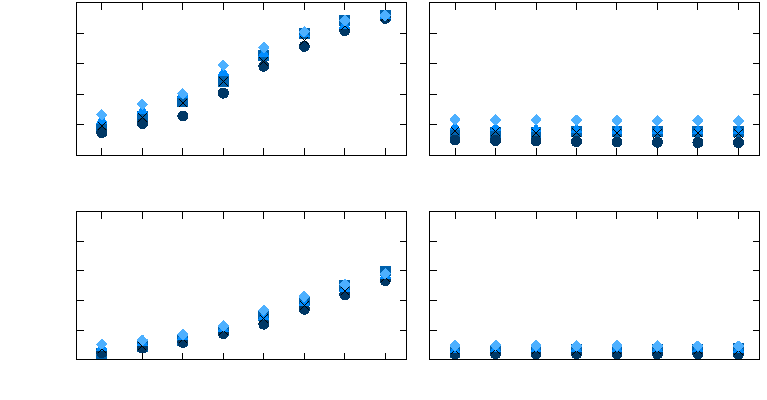
\includegraphics{uniform_results_2D}}%
    \gplfronttext
  \end{picture}%
\endgroup
